\documentclass[./../main.tex]{subfiles}
\graphicspath{{img/}}

\begin{document}
    \begin{exercise}[Cadena monoatómica con acoplamiento entre segundos vecinos]
        Considera una cadena unidimensional de átomos idénticos de masa \(m\). Cada átomo está unido con su vecino a través de un resorte de constante \(\kappa_{1}\). Considera además que cada átomo también está conectado con su segundo vecino por medio de un segundo resorte de constante \(\kappa_{2}\), como se ilustra en la \cref{fig:monoatomicChain}.

        \begin{figure}[htb]
            \centering
            % \includegraphics[height=0.3\textwidth, width=0.8\textwidth]{example-image-a}
            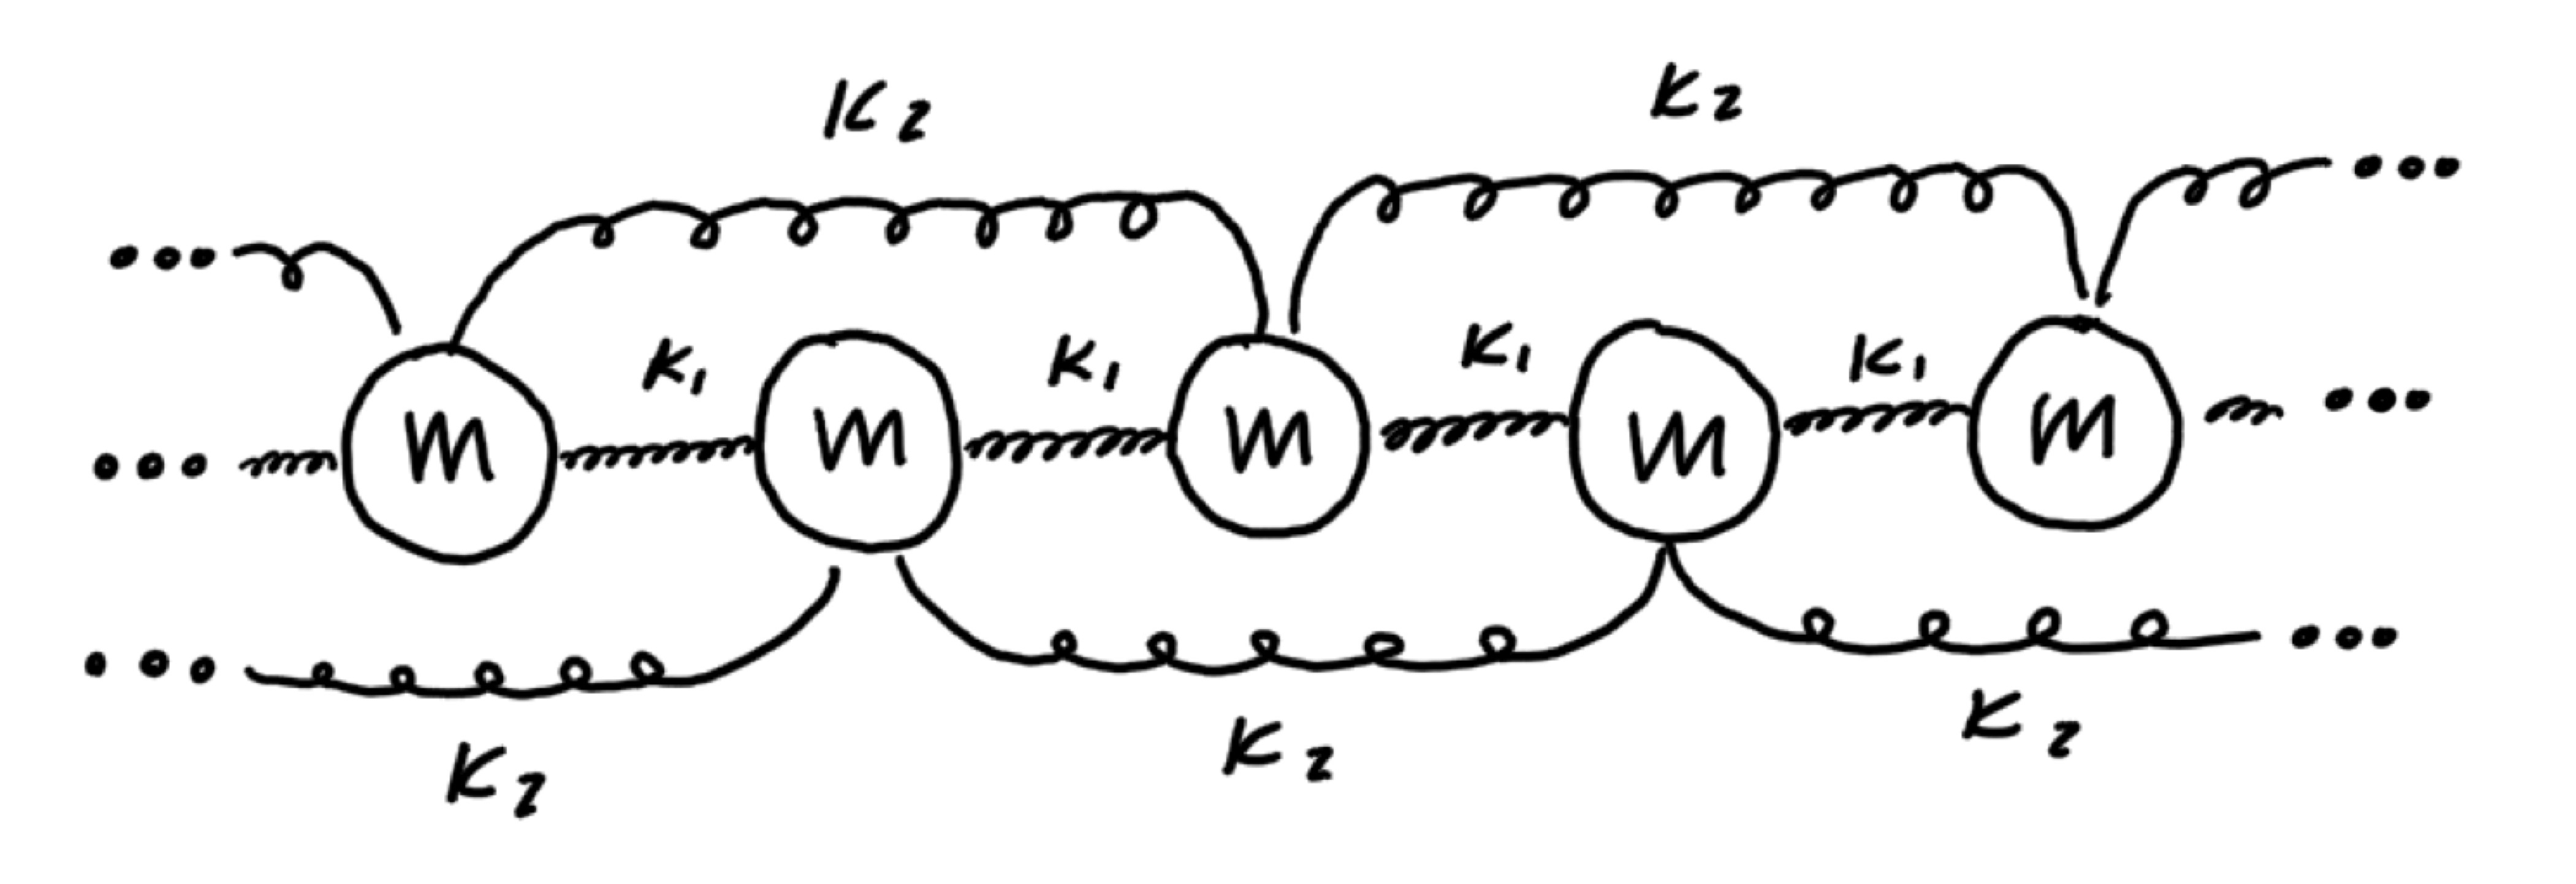
\includegraphics[width=0.6\textwidth]{monatomic-chain}
            \caption{Cadena monoatómica con acoplamiento entre primeros y segundos vecinos.}
            \label{fig:monoatomicChain}
        \end{figure}

        \begin{enumerate}
            \item (Valor: 2.5pt) - Muestra que la ecuación de movimiento asociada al desplazamiento \(\fdif{x_{n}}\), de la \(n\)-ésima masa es:
            
            \begin{equation*}
                m\fdif{\ddot{x}_{n}} = \kappa_{1}(\fdif{x_{n + 1}} - \fdif{x_{n}}) + \kappa_{1}(\fdif{x_{n - 1}} - \fdif{x_{n}}) + \kappa_{2}(\fdif{x_{n + 2}} - \fdif{x_{n}}) + \kappa_{2}(\fdif{x_{n - 2}} - \fdif{x_{n}})
            \end{equation*}

            \item (Valor: 2.5pt) - Usando el resultado del inciso anterior, demuestra que la relación de dispersión \(\omega(k)\) para este modelo está dada por:
            
            \begin{equation*}
                \omega(k) = \sqrt{\dfrac{2\kappa_{1}}{m}(1 - \cos(ka)) + \dfrac{2\kappa_{2}}{m}(1 - \cos(2ka))}
            \end{equation*}

            en donde \(a\) es la constante de la red (es decir, la separación entre átomos).

            \item (Valor: 2.5pt) - Grafica esta relación de dispersión dentro de la primera zona de Brillouin.
            \item (Valor: 2.5pt) - Usando el resultado del inciso (b), demuestra que la velocidad del sonido está dada por:
            
            \begin{equation*}
                v_{s} = a\sqrt{\dfrac{\kappa_{1} + 4\kappa_{2}}{m}}
            \end{equation*}
        \end{enumerate}
    \end{exercise}
\end{document}